\documentclass[11pt]{article}
\usepackage[margin=1in]{geometry}
\usepackage{cite}
\usepackage{amsmath,amssymb}
\usepackage{graphicx}
\usepackage{booktabs}
\usepackage{multirow}
\usepackage{url}
\usepackage[hidelinks]{hyperref}
\usepackage{enumitem}
\usepackage{xcolor}
\usepackage{float}
\usepackage{subcaption}
\usepackage{listings}

\lstdefinelanguage{Solidity}{
  keywords={pragma, solidity, contract, function, modifier, require, returns, return, mapping, address, uint, uint256, bool, string, bytes, public, private, internal, external, view, pure, payable, memory, storage, calldata, if, else, for, while, emit, event, struct, enum, import, is, new, delete, true, false, msg, block, tx, this},
  morecomment=[l]{//},
  morecomment=[s]{/*}{*/},
  morestring=[b]",
  morestring=[b]',
  sensitive=true,
}

\lstset{
  basicstyle=\footnotesize\ttfamily,
  breaklines=true,
  frame=single,
  numbers=left,
  numberstyle=\tiny\color{gray},
  numbersep=8pt,
  xleftmargin=15pt,
  tabsize=2,
  captionpos=b,
  keywordstyle=\bfseries,
  commentstyle=\itshape\color{gray},
}

\title{\textbf{Preliminary Project Report}\\[0.3cm]
\Large From Prompt to Exploit: An Empirical Study of\\Security Vulnerabilities in LLM-Generated Smart Contracts}

\author{Anik Tahabilder \& Dong Vo}

\date{March 31, 2026}

\begin{document}

\maketitle

%======================================================================
\section{Problem Statement and Motivation}
%======================================================================

Nowadays, developers are using Large Language Models (LLMs) like ChatGPT, Claude, and GitHub Copilot more and more to write code. This also includes writing Solidity smart contracts, which are programs that run on the Ethereum blockchain and often handle large amounts of money. In 2022 alone, over \$3.8 billion was stolen because of smart contract bugs~\cite{chainalysis2023}. A recent GitHub survey found that 92\% of developers now use some kind of AI coding tool~\cite{github_copilot}.

What makes smart contracts different from regular software is that once you deploy them on the blockchain, you cannot go back and fix them. If there is a vulnerability, anyone can see it and exploit it right away. There is no way to push a patch like you would for a web app. This makes the security of smart contract code extremely important.

The problem is, while there is some research on using LLMs to \emph{detect} vulnerabilities in smart contracts~\cite{gptscan, david2023you}, nobody has really looked at how many vulnerabilities LLMs actually \emph{introduce} when they generate smart contract code. On top of that, Perry et al.~\cite{perry2023users} showed that when developers use AI assistants, they actually write less secure code but think it is more secure. This is a dangerous combination.

Our project tries to fill this gap. We want to find out: when you ask different LLMs to write smart contracts, how many security vulnerabilities do they put in the code? Do some LLMs do better than others? And how does the generated code compare to what human developers write? We organized our study around three research questions:

\begin{enumerate}[leftmargin=*]
    \item \textbf{RQ1 (Prevalence \& Cross-LLM Comparison):} How common are security vulnerabilities in LLM-generated smart contracts, and do different LLMs produce significantly different levels of security?
    \item \textbf{RQ2 (Vulnerability Taxonomy \& LLM-Specific Patterns):} What types of vulnerabilities show up the most in LLM-generated contracts, and do LLMs exhibit distinct vulnerability patterns that are absent in human-written code?
    \item \textbf{RQ3 (Adversarial Prompts \& Human Baseline Comparison):} Do adversarial prompts that exploit LLM biases increase vulnerability rates, and how does LLM-generated code compare to real human-written contracts deployed on Ethereum?
\end{enumerate}

%======================================================================
\section{Brief Literature Review}
%======================================================================

\textbf{Security of LLM-Generated Code.}
There has been growing interest in understanding whether AI-generated code is secure. Pearce et al.~\cite{copilot_eval} conducted one of the earliest and most influential studies on this topic. They tested GitHub Copilot on 89 security-relevant scenarios based on the CWE (Common Weakness Enumeration) taxonomy and found that roughly 40\% of the generated code contained vulnerabilities. This was one of the first clear signals that AI coding tools can introduce real security problems. Building on this, Perry et al.~\cite{perry2023users} ran a controlled user study with 47 developers split into two groups -- one using an AI assistant and one without. They found that developers with AI assistants actually wrote \emph{less} secure code, but rated their own code as \emph{more} secure. This overconfidence effect is particularly worrying in the smart contract space where bugs can lead to immediate financial losses. Sandoval et al.~\cite{sandoval2023lost} confirmed similar findings in a larger study with professional developers, showing that this is not just a student effect.

Tony et al.~\cite{tony2023llmSecEval} created a benchmark called LLMSecEval with 150 natural language prompts covering 18 CWE types, which allows systematic evaluation of how different LLMs handle security-sensitive code generation. Tihanyi et al.~\cite{tihanyi2023formai} took a different approach and built FormAI, a large dataset of 112,000 AI-generated C programs with vulnerability labels obtained through dynamic analysis. Jesse et al.~\cite{jesse2023large} studied LLM code bugs more broadly and found that LLMs tend to make certain types of errors systematically rather than randomly.

However, all of these studies focus on general-purpose languages like C, Python, and JavaScript. Nobody has done this kind of large-scale study specifically for smart contracts. Smart contracts are a much higher-stakes domain because of immutability (you cannot patch them after deployment), direct financial exposure, and the adversarial nature of public blockchains where anyone can try to exploit a bug.

\textbf{Smart Contract Security Tools and Empirical Studies.}
The smart contract security tooling ecosystem has matured a lot over the past few years. Slither~\cite{slither} is currently the most widely used tool --- it performs fast static analysis and comes with over 90 built-in vulnerability detectors covering things like reentrancy, access control issues, and unchecked return values. Mythril~\cite{mythril} takes a different approach and uses symbolic execution, meaning it explores different execution paths through the code to find bugs that only show up under specific conditions. This makes it slower but able to catch deeper issues. Securify~\cite{securify} applies formal verification techniques to check contracts against predefined security patterns. Oyente~\cite{oyente} was one of the earliest symbolic execution tools for Ethereum and helped establish the field.

Durieux et al.~\cite{durieux2020empirical} conducted the most comprehensive comparison of smart contract analysis tools to date, testing 9 different tools on 47,587 contracts. Their most important finding was that no single tool catches all vulnerability types, and the tools have very low agreement with each other, meaning they each find different bugs. This directly motivated our decision to use three different tools (Slither, Mythril, and Semgrep) instead of relying on just one. Ren et al.~\cite{ren2021empirical} analyzed 21,212 real-world deployed contracts to establish baseline numbers for how common different vulnerability types are in practice. SmartBugs~\cite{smartbugs} provides a curated and labeled dataset that researchers use to benchmark new tools.

\textbf{LLMs for Vulnerability Detection.}
There is a parallel line of work that uses LLMs to \emph{find} bugs in smart contracts rather than generate code. GPTScan~\cite{gptscan} combines GPT-4 with traditional static analysis to detect logic vulnerabilities, and showed higher precision than either approach alone. SmartLLMSentry~\cite{smartllmsentry} uses LLMs with chain-of-thought reasoning to detect vulnerabilities step by step. PropertyGPT~\cite{propertygpt} uses LLMs to automatically generate formal security properties that can then be verified. David et al.~\cite{david2023you} tested ChatGPT's ability to both detect and repair smart contract bugs, finding moderate detection accuracy (about 68\%) but poor repair success rates. ContractTinker~\cite{contracttinker} proposed using LLMs for automated smart contract repair.

These works are closely related but fundamentally different from ours. They study LLMs as \emph{detectors} of existing bugs, while we study LLMs as \emph{sources} of new bugs. An interesting implication of combining both perspectives is the possibility of circular vulnerabilities: an LLM that generates vulnerable code might also fail to detect those same types of vulnerabilities when asked to review the code.

\textbf{Adversarial Attacks on LLMs.}
Researchers have shown that LLMs can be manipulated to produce harmful output in various ways. Prompt injection~\cite{perez2022ignore} and jailbreaking~\cite{kang2024exploiting} attacks demonstrate that LLMs can be tricked into ignoring their safety guidelines. In the code domain specifically, Schuster et al.~\cite{schuster2021you} showed that poisoning the training data can cause code completion tools to systematically suggest vulnerable code patterns. Wan et al.~\cite{wan2023poisoning} extended this to instruction-tuned models and showed that even subtle training data manipulation can cause models to consistently produce specific types of vulnerabilities.

Our adversarial prompt approach is different from these prior works in two ways. First, we focus on prompt-level manipulation rather than training data poisoning, which is a more realistic threat model since most developers do not have access to modify training data. Second, our adversarial prompts are designed to look natural and plausible --- they look like requests a regular developer might actually type, such as ``optimize this for gas efficiency'' or ``keep the implementation minimal.'' This is important because our results show that you do not need sophisticated prompt engineering to get vulnerable code --- even normal-sounding requests produce insecure contracts.

%======================================================================
\section{Methodology and Plan of Action}
%======================================================================

Our project has four main phases. Figure~\ref{fig:pipeline_overview} gives an overview.

\begin{figure}[H]
    \centering
    \fbox{\parbox{0.9\columnwidth}{\centering
    \textbf{Phase 1: Dataset Generation} (2,400 contracts from 8 LLMs) \\
    $\downarrow$ \\
    \textbf{Phase 2: Vulnerability Analysis} (Slither + Mythril + Semgrep) \\
    $\downarrow$ \\
    \textbf{Phase 3: Human Baseline Collection} (241 real Ethereum contracts) \\
    $\downarrow$ \\
    \textbf{Phase 4: Statistical Analysis \& Manual Validation}
    }}
    \caption{Overview of our four-phase research pipeline.}
    \label{fig:pipeline_overview}
\end{figure}

\subsection{Phase 1: Dataset Generation {\normalfont\textit{(Complete)}}}

We picked eight LLMs that cover both general-purpose models and code-specialized models. Table~\ref{tab:llm_config} shows the details.

\begin{table}[H]
\centering
\caption{LLM Selection and Configuration}
\label{tab:llm_config}
\resizebox{\columnwidth}{!}{%
\begin{tabular}{@{}llccc@{}}
\toprule
\textbf{Model} & \textbf{Type} & \textbf{Access} & \textbf{Temp.} & \textbf{Contracts} \\
\midrule
GPT-4o & General-purpose & OpenAI API & 0.7 & 300 \\
GPT-5 & General-purpose & OpenAI API & 1.0$^\dagger$ & 300 \\
Claude 3.5 Sonnet & General-purpose & Anthropic CLI & 0.7 & 300 \\
Gemini 2.5 Flash-Lite & General-purpose & Google API & 0.7 & 300 \\
\midrule
DeepSeek Coder V2 & Code-specialized & Ollama (local) & 0.7 & 300 \\
Qwen 2.5 Coder 32B & Code-specialized & Ollama (local) & 0.7 & 300 \\
CodeLlama-34B & Code-specialized & Ollama (local) & 0.7 & 300 \\
Codestral 22B & Code-specialized & Ollama (local) & 0.7 & 300 \\
\bottomrule
\multicolumn{5}{l}{\scriptsize $^\dagger$GPT-5 does not support configurable temperature.}
\end{tabular}%
}
\end{table}

We asked each LLM to generate 300 contracts across 20 different categories (things like ERC-20 tokens, DeFi staking, governance, cross-chain bridges, flash loans, etc.) at three complexity levels. Half the prompts were standard and half were adversarial, meaning they were designed to push the LLM toward cutting corners, like asking it to optimize for gas efficiency or keep things simple. In total, we got \textbf{2,400 contracts}.

For the commercial models (GPT-4o, GPT-5, Claude, Gemini), we used their APIs. For the open-source models (DeepSeek, Qwen, CodeLlama, Codestral), we ran them locally using Ollama on machines with NVIDIA A6000 and RTX 3090 GPUs.

\subsection{Phase 2: Vulnerability Analysis {\normalfont\textit{(Complete)}}}

We ran all 2,400 contracts through three security analysis tools:
\begin{itemize}[leftmargin=*]
    \item \textbf{Slither}~\cite{slither}: A fast static analyzer with 90+ detectors. We ran it on all 2,400 contracts. Out of these, 1,566 compiled successfully.
    \item \textbf{Mythril}~\cite{mythril}: A symbolic execution tool that can catch deeper bugs. Since it is very slow (about 5 minutes per contract), we ran it on a stratified sample of 499 contracts. 408 of them completed successfully.
    \item \textbf{Semgrep}: We wrote custom rules for Solidity-specific patterns and ran them on all 2,400 contracts.
\end{itemize}

After running all three tools, we deduplicated the results (to avoid counting the same bug twice from different tools) and mapped each finding to a CWE identifier. This gave us \textbf{5,134 unique vulnerabilities} across the compiled contracts.

\subsection{Phase 3: Human Baseline {\normalfont\textit{(Complete)}}}

To have something to compare against, we collected 241 verified smart contracts from Ethereum mainnet through Etherscan. These are real contracts from well-known protocols like Uniswap, Aave, Compound, Gnosis Safe, and Lido. We flattened them using Foundry's \texttt{forge flatten} tool (to resolve multi-file imports) and then ran the same analysis pipeline on them.

\subsection{Phase 4: Statistical Analysis {\normalfont\textit{(In Progress)}}}

We already ran all the statistical tests: Kruskal-Wallis for comparing across LLMs, Mann-Whitney U for pairwise comparisons, Cliff's delta for effect sizes, and bootstrap confidence intervals. What is still left is the manual validation part: we are going through 120 randomly sampled contracts by hand to check how accurate the tools are (how many findings are real bugs vs. false alarms).

%======================================================================
\section{Preliminary Results}
%======================================================================

Most of our analysis is done. Below are the key findings.

\subsection{RQ1: Vulnerability Prevalence and Cross-LLM Comparison}

\textbf{Finding: 64.5\% of compilable LLM-generated contracts have at least one vulnerability, with significant differences across LLMs.}

Out of 2,400 generated contracts, 1,566 (65.2\%) compiled successfully. The compilation rates were very different across models; GPT-5 compiled 91.0\% of its contracts, while CodeLlama only managed 34.7\%. This by itself is an interesting finding that nobody has reported before.

\begin{figure}[H]
    \centering
    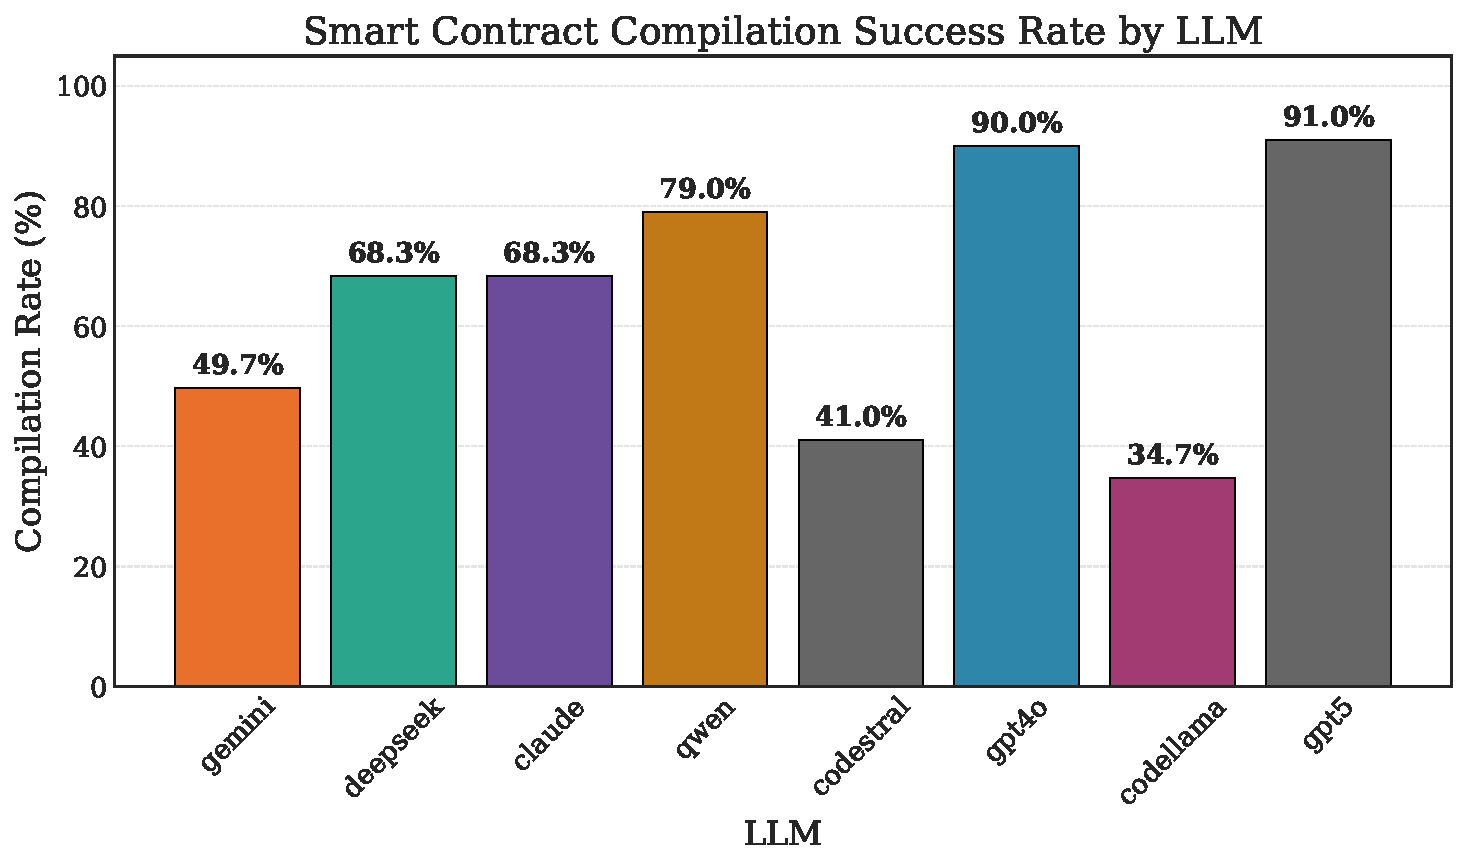
\includegraphics[width=\columnwidth]{visualization/figures/fig10_compilation_rates.pdf}
    \caption{Compilation rates by LLM. The commercial models (GPT-5, GPT-4o) compile much better than the open-source code models (CodeLlama, Codestral).}
    \label{fig:compilation}
\end{figure}

Looking at the compiled contracts, our tools found a total of \textbf{5,134 vulnerabilities}. Table~\ref{tab:overall} breaks them down by severity.

\begin{table}[H]
\centering
\caption{Vulnerability Prevalence ($n=1{,}566$ compiled contracts)}
\label{tab:overall}
\begin{tabular}{@{}lrrr@{}}
\toprule
\textbf{Severity} & \textbf{Count} & \textbf{\% of Total} & \textbf{Contracts Affected} \\
\midrule
High & 804 & 15.7\% & 419 (26.8\%) \\
Medium & 1,743 & 34.0\% & 597 (38.1\%) \\
Low & 2,587 & 50.4\% & 871 (55.6\%) \\
\midrule
\textbf{Total} & \textbf{5,134} & \textbf{100\%} & \textbf{1,010 (64.5\%)} \\
\bottomrule
\end{tabular}
\end{table}

The most concerning number here is that 26.8\% of contracts have high-severity vulnerabilities, the kind that could lead to someone losing money if the contract was deployed.

\subsubsection{Cross-LLM Comparison}

Not all LLMs are equal when it comes to security. A Kruskal-Wallis test confirms that the differences across LLMs are statistically significant ($H = 323.8$, $p < 10^{-65}$). Table~\ref{tab:llm_vulns} shows the vulnerability numbers for each LLM, counting only compiled contracts.

\begin{table}[H]
\centering
\caption{Per-LLM Vulnerability Statistics (Compiled Contracts Only)}
\label{tab:llm_vulns}
\resizebox{\columnwidth}{!}{%
\begin{tabular}{@{}lcccccc@{}}
\toprule
\textbf{LLM} & \textbf{$n$} & \textbf{Mean} & \textbf{Median} & \textbf{\% w/ Vuln} & \textbf{\% High-Sev} & \textbf{Vulns/100 LOC} \\
\midrule
Claude 3.5 Sonnet & 205 & 7.64 & 6 & 84.9\% & 33.7\% & 6.98 \\
Gemini 2.5 Flash-Lite & 149 & 4.52 & 3 & 80.5\% & 30.9\% & \textbf{8.43} \\
GPT-4o & 270 & 3.05 & 2 & 73.0\% & 29.3\% & 6.61 \\
DeepSeek Coder V2 & 205 & 2.98 & 2 & 73.2\% & 29.8\% & 7.96 \\
Qwen 2.5 Coder & 237 & 2.75 & 2 & 66.2\% & 28.7\% & 6.95 \\
GPT-5 & 273 & 1.79 & 0 & 35.5\% & 17.2\% & \textbf{2.22} \\
Codestral 22B & 123 & 1.57 & 1 & 52.0\% & 30.1\% & 6.88 \\
CodeLlama-34B & 104 & 1.23 & 0 & 49.0\% & 11.5\% & 5.16 \\
\bottomrule
\end{tabular}%
}
\end{table}

\begin{figure}[H]
    \centering
    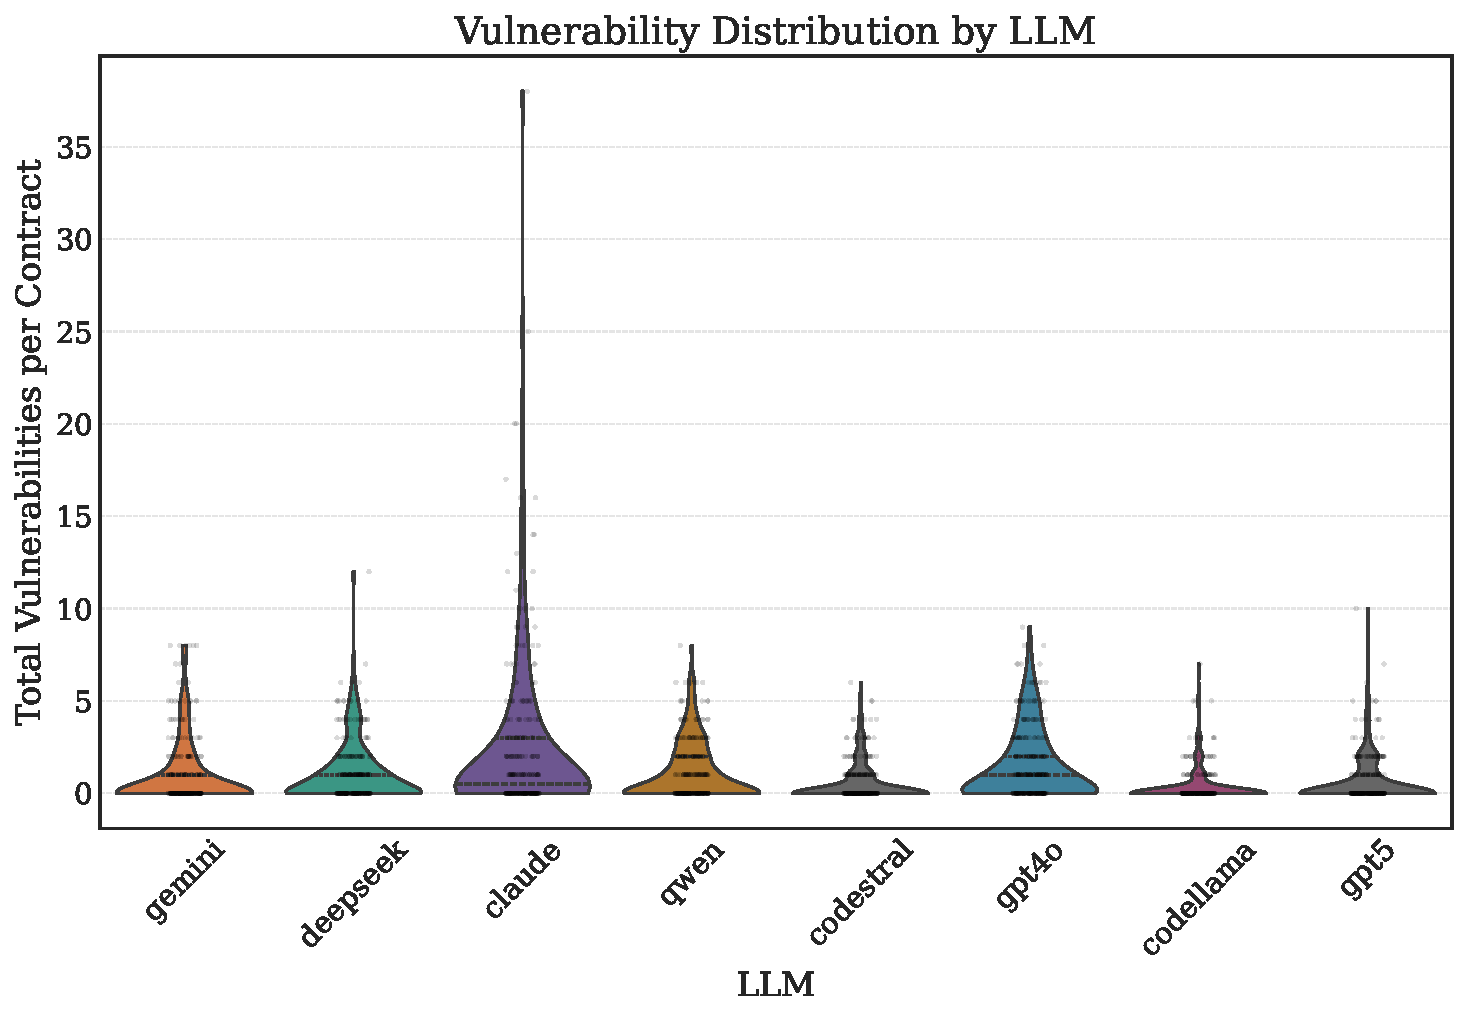
\includegraphics[width=\columnwidth]{visualization/figures/fig1_vulnerabilities_by_llm.pdf}
    \caption{Vulnerability distribution across LLMs. Claude has the highest raw count but also writes the longest contracts. GPT-5 has the fewest vulnerabilities relative to code size.}
    \label{fig:boxplot}
\end{figure}

At first glance, Claude looks like the worst because it averages 7.64 vulnerabilities per contract. But Claude also generates the biggest contracts (mean 113 lines of code). When we normalize by lines of code, the picture changes: Gemini actually has the worst vulnerability density at 8.43 vulns per 100 lines, while GPT-5 is the best at only 2.22 vulns per 100 lines.

\begin{figure}[H]
    \centering
    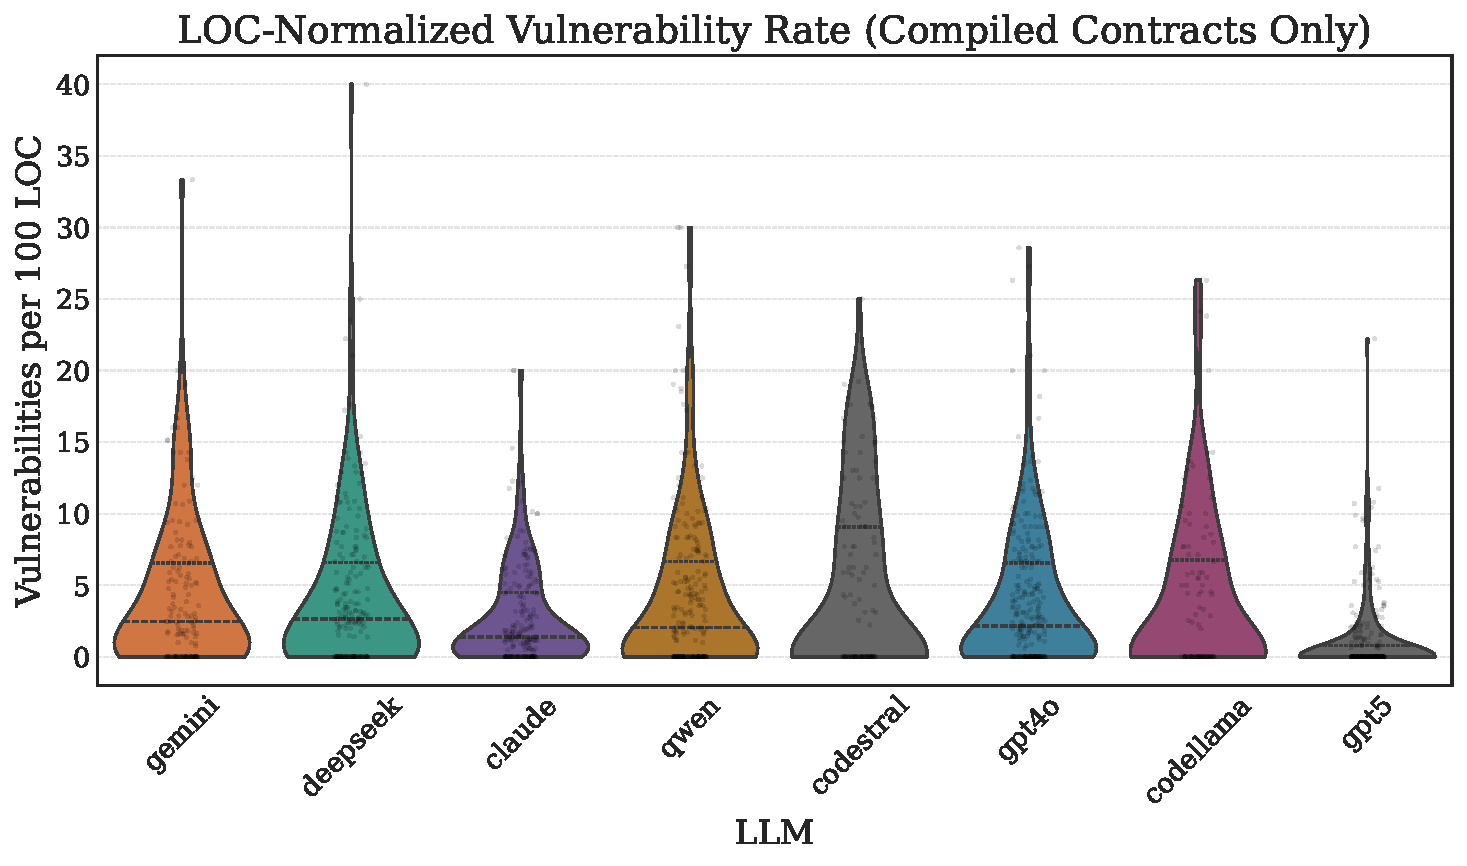
\includegraphics[width=\columnwidth]{visualization/figures/fig8_loc_normalized_violin.pdf}
    \caption{Vulnerability rate normalized by code size (vulns per 100 lines of code). This gives a fairer comparison since some LLMs write much longer contracts than others.}
    \label{fig:loc_normalized}
\end{figure}

GPT-5 is clearly the best model overall: it has the highest compilation rate (91.0\%) and the lowest vulnerability density (2.22/100 LOC). We also tested whether general-purpose models are better than code-specialized ones. Interestingly, when you normalize by code size, there is no significant difference (6.66 vs.\ 6.97 vulns/100 LOC, $p = 0.094$). The differences between individual models matter much more than whether a model is ``general-purpose'' or ``code-specialized.''

\subsection{RQ2: Vulnerability Types and LLM-Specific Patterns}

\subsubsection{Vulnerability Taxonomy}

\textbf{Finding: Reentrancy and timestamp dependence are the most common vulnerability types.}

Table~\ref{tab:taxonomy} shows the top vulnerability types we found, mapped to their CWE identifiers.

\begin{table}[H]
\centering
\caption{Top Vulnerability Types (Mapped to CWE)}
\label{tab:taxonomy}
\small
\begin{tabular}{@{}rlrr@{}}
\toprule
\textbf{\#} & \textbf{Vulnerability Type} & \textbf{CWE} & \textbf{Count} \\
\midrule
1 & Timestamp Dependence & 829 & 1,865 \\
2 & Reentrancy & 841 & 1,201 \\
3 & Unchecked Return Value & 252 & 461 \\
4 & Missing Access Control & 284 & 153 \\
5 & Uninitialized State & 909 & 35 \\
6 & Weak Randomness & 330 & 4 \\
7 & tx.origin Authentication & 477 & 1 \\
\bottomrule
\end{tabular}
\end{table}

Timestamp dependence and reentrancy together make up 59.7\% of all findings. Reentrancy is especially dangerous because it is the vulnerability behind many of the biggest DeFi hacks in history (including the famous DAO hack in 2016).

\begin{figure}[H]
    \centering
    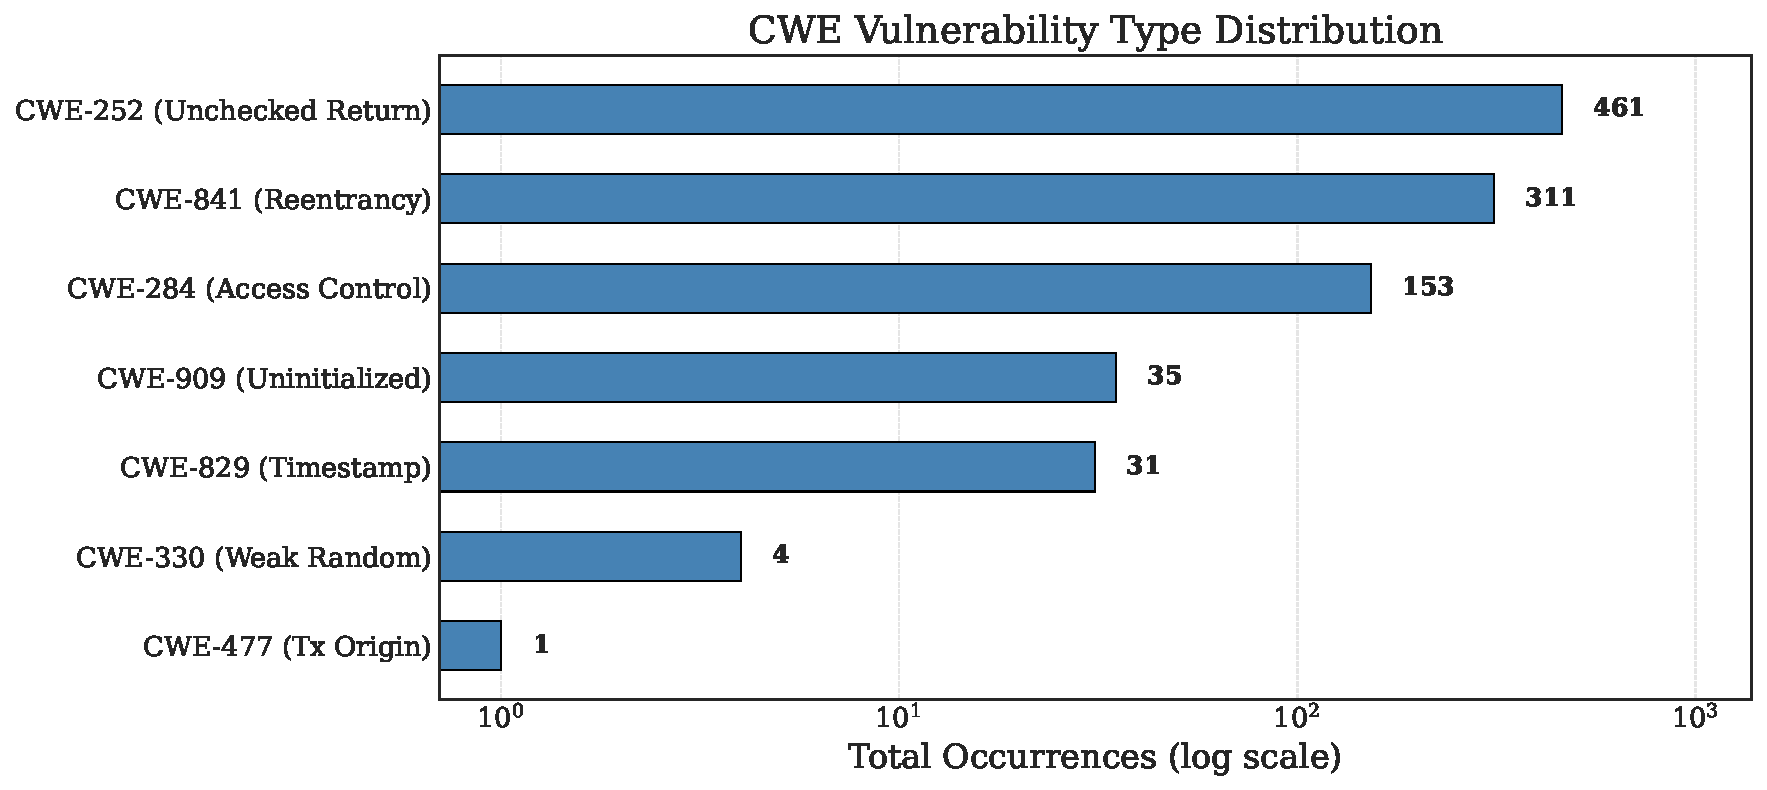
\includegraphics[width=\columnwidth]{visualization/figures/fig6_cwe_distribution.pdf}
    \caption{Distribution of vulnerability types (by CWE). Timestamp dependence and reentrancy dominate.}
    \label{fig:cwe_dist}
\end{figure}

\subsubsection{LLM-Specific Vulnerability Patterns}

\textbf{Finding: LLMs make three kinds of mistakes that human developers typically do not.}

\textbf{1. Phantom Guards.} Sometimes LLMs write a security modifier like \texttt{nonReentrant} but leave the body empty. The modifier name makes it \emph{look} like the function is protected, but it actually does nothing. This is especially sneaky because a code reviewer might glance at it and think the protection is there.

\begin{lstlisting}[language=Solidity, basicstyle=\scriptsize\ttfamily, caption={Phantom Guard pattern: the modifier name says ``nonReentrant'' but there is no actual locking logic inside.}]
// LLM-generated (VULNERABLE)
modifier nonReentrant() {
    _; // No lock! Just runs the function body
}
function withdraw(uint amt) nonReentrant {
    payable(msg.sender).call{value: amt}("");
    balances[msg.sender] -= amt;
}
\end{lstlisting}

\textbf{2. Unnecessary Reimplementations.} When we tell the LLM not to use external libraries, it tries to rewrite things like SafeMath by hand. But since Solidity 0.8.0 already has built-in overflow protection, this is unnecessary and can introduce subtle bugs. We found this in 4.0\% of contracts targeting Solidity 0.8+, especially from DeepSeek (9.7\%) and Gemini (8.7\%).

\textbf{3. Context Window Degradation.} In longer contracts (over 100 lines), the LLM tends to get sloppy toward the end. We measured this and found that risky code patterns show up 4.13$\times$ more often in the second half of long contracts compared to the first half. DeepSeek has the worst degradation (14.1$\times$). This makes sense because as the LLM generates more tokens, it loses track of the security patterns it was following earlier.

\subsection{RQ3: Adversarial Prompts and Human Baseline Comparison}

\subsubsection{Adversarial Prompts}

\textbf{Finding: Surprisingly, adversarial prompts do not increase vulnerability rates.}

This was our most unexpected result. We thought that prompts designed to push the LLM toward cutting corners (like ``optimize for gas'' or ``keep it minimal'') would result in more vulnerabilities. But that is not what happened. The Mann-Whitney U test gives $p = 0.997$ with a negligible effect size (Cliff's $\delta = -0.090$). If anything, standard prompts produce slightly \emph{more} vulnerabilities (mean 4.05 vs.\ 3.00), but this is simply because standard prompts lead to bigger contracts with more code.

\begin{figure}[H]
    \centering
    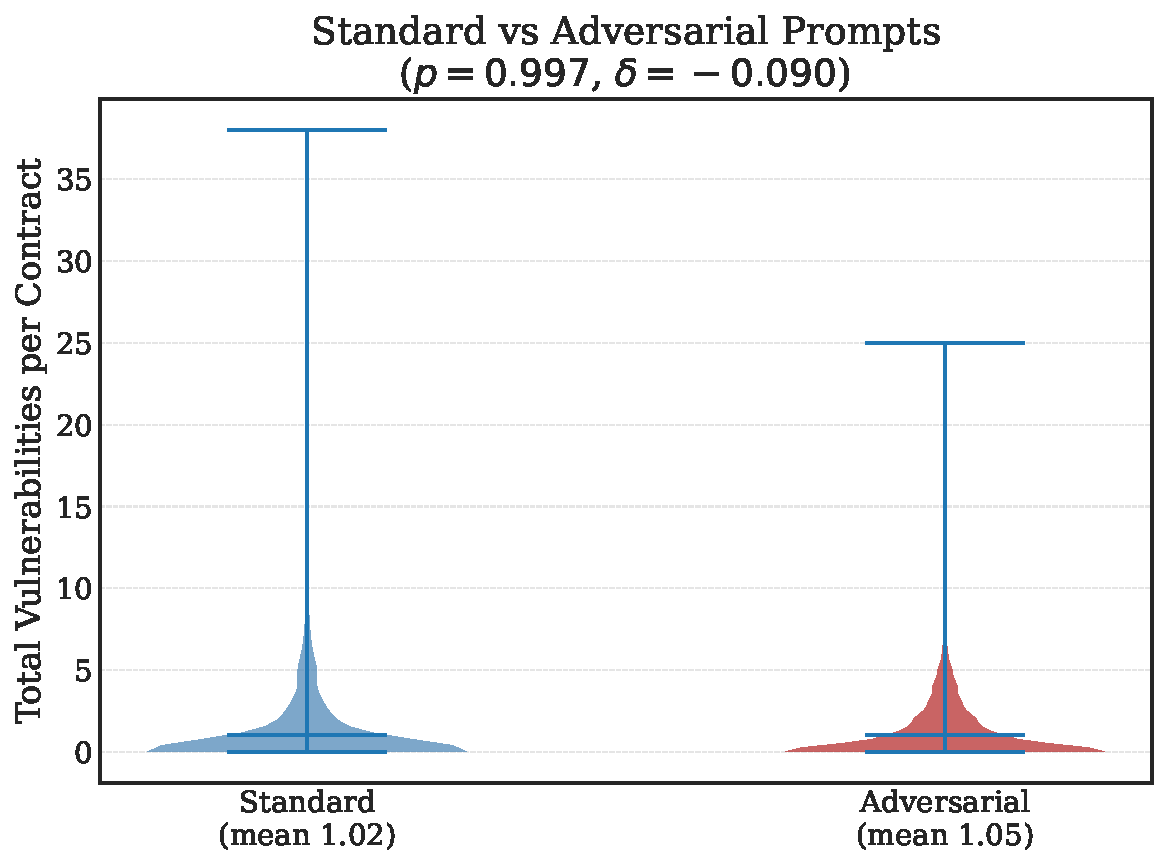
\includegraphics[width=\columnwidth]{visualization/figures/fig2_standard_vs_adversarial.pdf}
    \caption{Standard vs.\ adversarial prompts. The distributions look almost identical. Adversarial prompting does not make the code less secure.}
    \label{fig:adversarial}
\end{figure}

What this means is that the vulnerabilities are \emph{built into} how LLMs generate code; they come from the training data, not from the prompt. You cannot just write a better prompt and get secure code. Post-generation security analysis is the only reliable way to catch these bugs.

\subsubsection{Comparison with Human-Written Code}

We compared our LLM results against 241 verified contracts from Ethereum mainnet (from protocols like Uniswap, Aave, Compound, Gnosis Safe, and Lido). Table~\ref{tab:human} shows the comparison.

\begin{table}[H]
\centering
\caption{LLM-Generated vs.\ Human-Written Contracts}
\label{tab:human}
\begin{tabular}{@{}lcc@{}}
\toprule
\textbf{Metric} & \textbf{Human} & \textbf{LLM (8 models)} \\
\midrule
Total contracts & 241 & 2,400 \\
Compiled & 132 (54.8\%) & 1,566 (65.2\%) \\
With vulnerabilities & 82.6\% & 64.5\% \\
Mean findings/contract & 11.51 & 3.28 \\
Mean LOC & 446.7 & 52.3 \\
\textbf{Vulns/100 LOC} & \textbf{2.69} & \textbf{2.22--8.43} \\
High-sev \% of findings & 16.0\% & 15.7\% \\
\bottomrule
\end{tabular}
\end{table}

The raw numbers make it look like human contracts have more bugs (mean 11.51 vs.\ 3.28 per contract). But human contracts are also much bigger, averaging 446.7 lines on average compared to 52.3 for LLM code. When we normalize by code size, the vulnerability density is actually similar: 2.69 vulns/100 LOC for humans vs.\ 2.22--8.43 for different LLMs. The high-severity proportions are also almost identical (16.0\% vs.\ 15.7\%).

\begin{figure}[H]
    \centering
    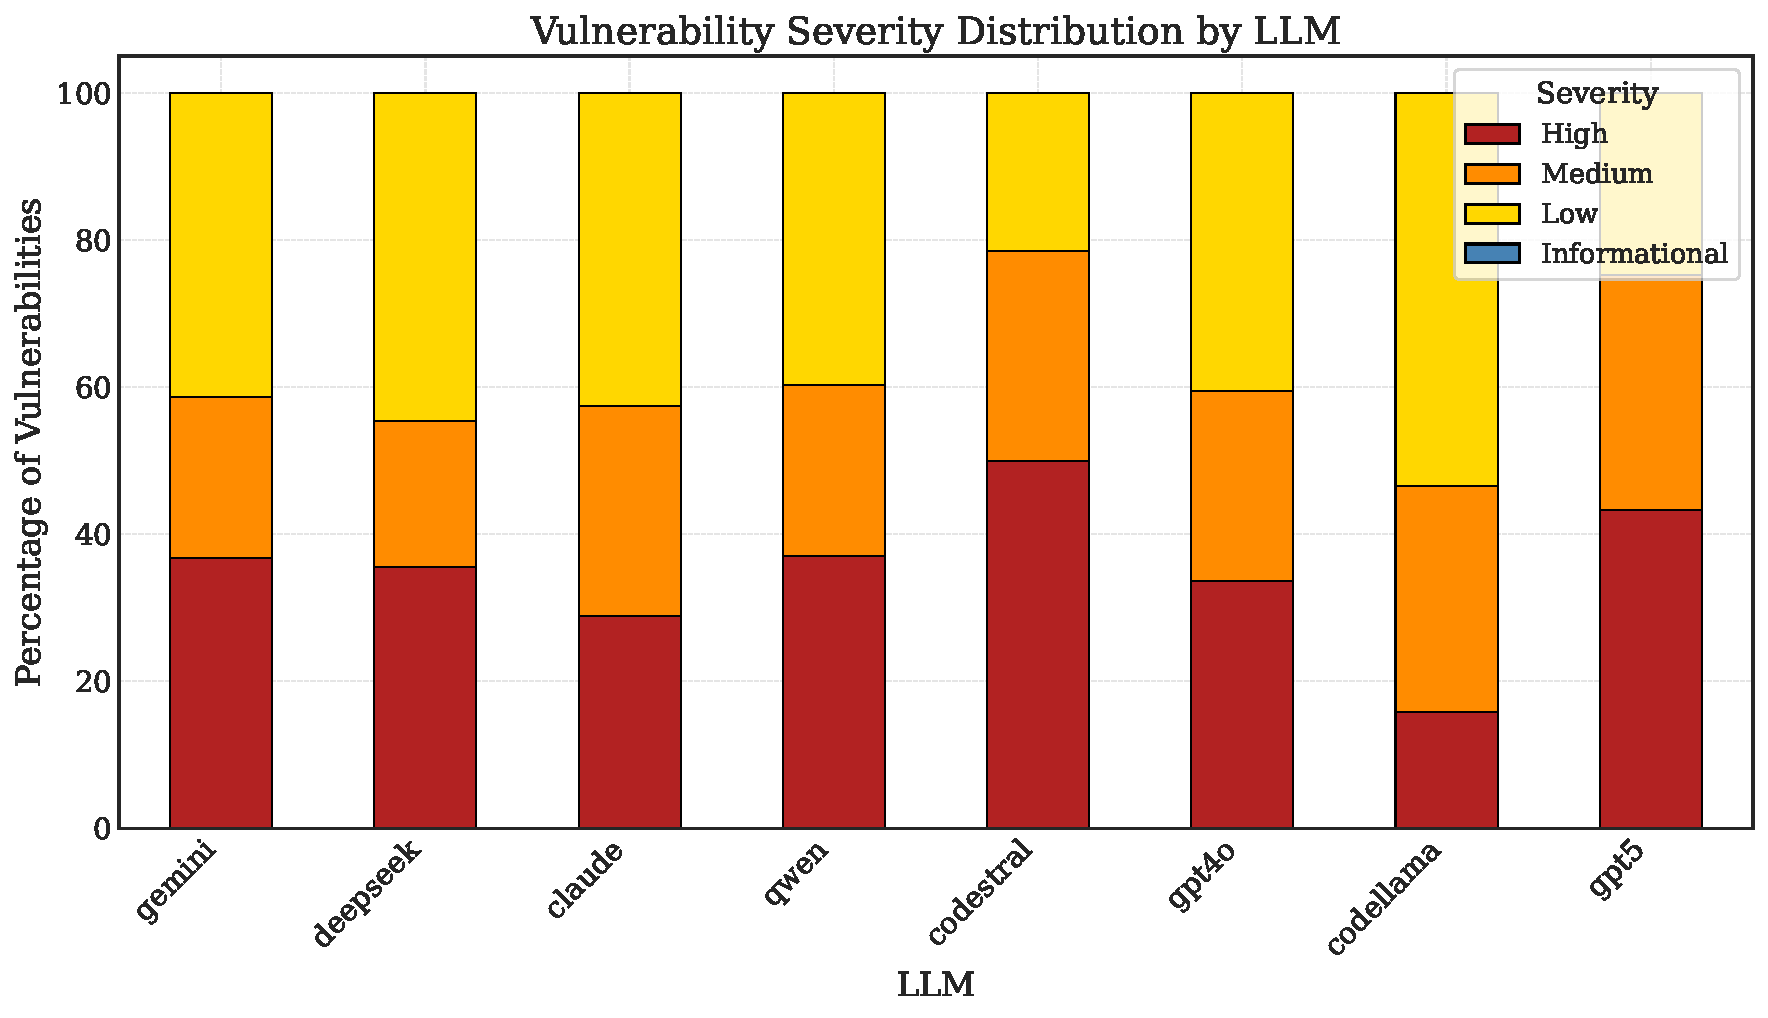
\includegraphics[width=\columnwidth]{visualization/figures/fig4_severity_distribution.pdf}
    \caption{Severity breakdown across LLMs. The proportion of high-severity findings is similar across all models and comparable to the human baseline.}
    \label{fig:severity}
\end{figure}

The big takeaway here is that LLM-generated code is not necessarily \emph{worse} than human code in terms of vulnerability density. The real problem is what happens \emph{after} the code is generated. Human-written contracts that are deployed on mainnet have gone through professional audits, extensive testing, and monitoring. When developers use LLM output, they often skip all of that. The danger is not the code quality itself but rather the security infrastructure that gets bypassed.

%======================================================================
\section{Remaining Work}
%======================================================================

Most of the heavy lifting is done. Here is what we still need to do:

\begin{enumerate}[leftmargin=*]
    \item \textbf{Manual Validation:} We are currently going through 120 randomly sampled contracts by hand to check how many of the tool findings are real bugs vs.\ false positives. This will let us report precision and recall numbers for our analysis pipeline.
    \item \textbf{Detector Filtering:} Some of the tool detectors produce a lot of noise (e.g., timestamp dependence and benign reentrancy warnings). We need to filter these out to get cleaner vulnerability counts.
    \item \textbf{Writing and Revisions:} Once the manual validation is done, we will update the numbers in the paper, polish the figures, and incorporate feedback from this preliminary report.
    \item \textbf{Reproducibility Package:} We plan to release the full dataset (all 2,400 contracts with prompts), the analysis scripts, and documentation so other researchers can reproduce our work.
\end{enumerate}

%======================================================================

\begin{thebibliography}{20}

\bibitem{github_copilot} GitHub, ``Survey reveals AI's impact on the developer experience,'' GitHub Blog, 2023.

\bibitem{chainalysis2023} Chainalysis, ``The 2023 Crypto Crime Report,'' Chainalysis Inc., 2023.

\bibitem{gptscan} Y.~Sun et al., ``GPTScan: Detecting Logic Vulnerabilities in Smart Contracts by Combining GPT with Program Analysis,'' in \textit{Proc.\ ICSE}, 2024.

\bibitem{david2023you} D.~David et al., ``Do You Still Need a Manual Smart Contract Audit?'' arXiv:2306.12338, 2023.

\bibitem{perry2023users} N.~Perry et al., ``Do Users Write More Insecure Code with AI Assistants?'' in \textit{Proc.\ CCS}, 2023.

\bibitem{copilot_eval} H.~Pearce et al., ``Asleep at the Keyboard? Assessing the Security of GitHub Copilot's Code Contributions,'' in \textit{Proc.\ IEEE S\&P}, 2022.

\bibitem{tony2023llmSecEval} C.~Tony et al., ``LLMSecEval: A Dataset of Natural Language Prompts for Security Evaluations,'' in \textit{Proc.\ MSR}, 2023.

\bibitem{tihanyi2023formai} N.~Tihanyi et al., ``FormAI -- A Dataset of 112,000 AI-Generated C Programs with Vulnerability Classification,'' arXiv:2307.02192, 2023.

\bibitem{slither} J.~Feist et al., ``Slither: A Static Analysis Framework for Smart Contracts,'' in \textit{Proc.\ WETSEB}, 2019.

\bibitem{mythril} C.~Mueller, ``Mythril: Security analysis tool for EVM bytecode,'' GitHub, 2018.

\bibitem{durieux2020empirical} T.~Durieux et al., ``Empirical Review of Automated Analysis Tools on 47,587 Ethereum Smart Contracts,'' in \textit{Proc.\ ICSE}, 2020.

\bibitem{ren2021empirical} M.~Ren et al., ``Empirical Evaluation of Smart Contract Testing: What Is the Best Choice?'' in \textit{Proc.\ ISSTA}, 2021.

\bibitem{schuster2021you} R.~Schuster et al., ``You Autocomplete Me: Poisoning Vulnerabilities in Neural Code Completion,'' in \textit{Proc.\ USENIX Security}, 2021.

\bibitem{kang2024exploiting} D.~Kang et al., ``Exploiting Programmatic Behavior of LLMs: Dual-Use Through Standard Security Attacks,'' in \textit{Proc.\ IEEE S\&P}, 2024.

\bibitem{sandoval2023lost} G.~Sandoval et al., ``Lost at C: A User Study on the Security Implications of Large Language Model Code Assistants,'' in \textit{Proc.\ USENIX Security}, 2023.

\bibitem{jesse2023large} K.~Jesse et al., ``Large Language Models and Simple, Stupid Bugs,'' in \textit{Proc.\ MSR}, 2023.

\bibitem{securify} P.~Tsankov et al., ``Securify: Practical Security Analysis of Smart Contracts,'' in \textit{Proc.\ CCS}, 2018.

\bibitem{oyente} L.~Luu et al., ``Making Smart Contracts Smarter,'' in \textit{Proc.\ CCS}, 2016.

\bibitem{smartbugs} T.~Durieux et al., ``SmartBugs: A Framework to Analyze Solidity Smart Contracts,'' in \textit{Proc.\ ASE}, 2020.

\bibitem{smartllmsentry} Y.~Zhang et al., ``SmartLLMSentry: LLM-based Smart Contract Vulnerability Detection,'' arXiv, 2024.

\bibitem{propertygpt} Z.~Liu et al., ``PropertyGPT: LLM-driven Formal Verification of Smart Contracts through Retrieval-Augmented Property Generation,'' arXiv, 2024.

\bibitem{contracttinker} W.~Chen et al., ``ContractTinker: LLM-Empowered Vulnerability Repair for Real-World Smart Contracts,'' arXiv, 2024.

\bibitem{perez2022ignore} F.~Perez and I.~Ribeiro, ``Ignore This Title and HackAPrompt: Exposing Systemic Weaknesses of LLMs through a Global Scale Prompt Hacking Competition,'' arXiv:2311.16119, 2023.

\bibitem{wan2023poisoning} Y.~Wan et al., ``Poisoning Language Models During Instruction Tuning,'' in \textit{Proc.\ ICML}, 2023.

\end{thebibliography}

\end{document}
